\documentclass[11pt,a4paper]{article}
\usepackage[left=2.5cm,right=2cm, bottom=2cm]{geometry}
\usepackage[utf8]{inputenc}
\usepackage{amsmath}
\usepackage{amsfonts}
\usepackage{amssymb}
\usepackage{amsfonts}
\usepackage{amsmath}
\usepackage{graphicx}
\usepackage{subfigure}
\usepackage{color}
\usepackage{abstract}
\usepackage{float}
\usepackage[toc,page]{appendix}
\usepackage{hyperref}
\usepackage{fancyhdr}
\usepackage{algorithm} 
\usepackage{algpseudocode} 
\usepackage{listings}
\usepackage{xcolor} % for setting colors
% set the default code style
\lstset{
	frame=tb, % draw a frame at the top and bottom of the code block
	tabsize=4, % tab space width
	showstringspaces=false, % don't mark spaces in strings
	numbers=left, % display line numbers on the left
	commentstyle=\color{green}, % comment color
	keywordstyle=\color{blue}, % keyword color
	stringstyle=\color{red} % string color
}

\pagestyle{fancy}
\fancyhf{}
\rhead{\today}
\lhead{\bfseries Alexander Leitner 01525882}
\rfoot{}



\begin{document}
\begin{center}
	\fontsize{24pt}{10pt}\selectfont
	\textsc{\textbf{Computational Science on Many-Core Architectures  Exercise 8}}
\end{center}
\section*{Example 1 Libraries (5 Points)}
\subsection*{a)}

\begin{center}
	\begin{minipage}[t]{0.5\textwidth}
		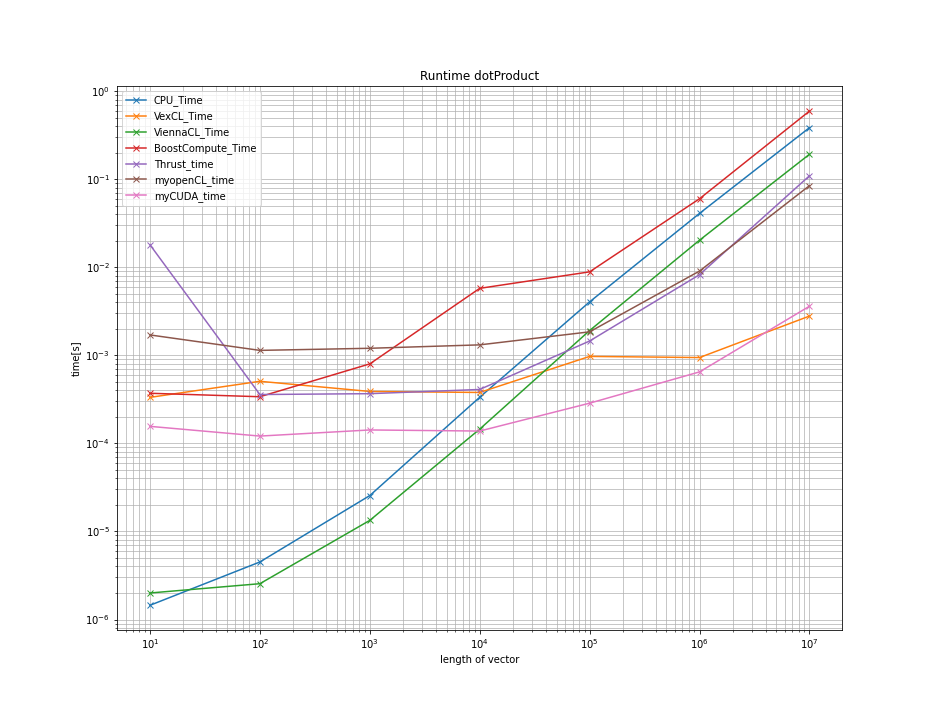
\includegraphics[width=\textwidth]{Bilder/Runtime_dotProduct}
	\end{minipage}
\end{center}

\begin{lstlisting}[language=C++, caption={opencl kernel}]
const char *my_opencl_program = ""
"__kernel void vec_mult(__global double *x,\n"
"                      __global double *y,\n"
"                      __global double *result,\n"
"                      unsigned int N\n)"
"{\n"
"  for (unsigned int i  = get_global_id(0);\n"
"                    i  < N;\n"
"                    i += get_global_size(0))\n"
"    result[i] = x[i] * y[i];\n"
"}"; 
\end{lstlisting}


\end{document}